\section{Obiettivo}
L'obiettivo di questo progetto è quello di realizzare un programma scritto in \textbf{OCaml} che risolva il \textit{problema} della \textit{colorazione di un grafo}: riuscire a colorare, se possibile, ogni nodo del grafo in modo da non avere mai nodi adiacenti con lo stesso colore. In via più formale, dato un grafo \lstinline[style=cmd]|g| ed un numero massimo di colori utilizzabili \lstinline[style=cmd]|N|, assegnare un colore ( da $0$ a $N-1$) ai nodi in modo tale che non esistano nodi adiacenti con lo stesso colore; qualora il numero di colori \lstinline[style=cmd]|N| non sia sufficiente per realizzare la colorazione, riportare un errore.
 
\section{Struttura del Progetto}
%TODO: aggiungere la struttura del progetto. forse va bene una foto o il risultato di un LS.
Di seguito sarà riportata la struttura delle cartelle e dei file del progetto con una breve descrizione per quelli più importanti. I file OCaml sono divisi in base al compito che svolgono le funzioni al loro interno (\textit{e.g.: \lstinline[style=cmd]|graphUtils| conterrà le funzioni che operano sui grafi, ecc.}) e sono sempre formati da un file \lstinline[style=cmd]|.ml| che contiene il copro della funzione con tutte le varie espressioni ed un file \lstinline[style=cmd]|.mli| nel quale è presente solo il tipo delle funzioni ed espressioni che verranno utilizzate dagli altri file. %TODO: rivedere meglio

\begin{figure}[H]
	\dirtree{%
		.1 .
		.1 Makefile.
		.1 src.
		.2 main.ml.
		.2 main.mli.
		.2 graphUtils.ml.
		.2 graphUtils.mli.
		.2 data.ml.
		.2 data.mli.
		.2 printer.ml.
		.2 printer.mli.
		.2 rappresentazione\_grafo.
		.3 rappresentazione\_grafo.py.
	}
	\caption{Rappresentazione schematizzata dei file e cartelle del progetto.}
\end{figure}

\begin{itemize}
	\item \lstinline[style=cmd]|Makefile|: utilizzato per compilare il progetto e generare l'eseguibile per avviarlo (vedere ...)	%TODO: aggiungere riferimento
	\item \lstinline[style=cmd]|main|: contiene la funzione principale che si occupa di avviare la colorazione e di gestire le scelte fatte dall'utente
	\item \lstinline[style=cmd]|graphUtils|: insieme di funzioni che operano sui grafi che svolgono l'effettivo compito di colorazione
	\item \lstinline[style=cmd]|data|: insieme di grafi per testare il corretto funzionamento del progetto. Questi possono essere aggiunti e rimossi in modo semplice ed efficiente
	\item \lstinline[style=cmd]|printer|: insieme di funzioni ed espressioni per stampare a video menu ed altri elementi con anche la presenza di colori ed emoji
	\item \lstinline[style=cmd]|rappresentazione\_grafo|: script in python per rappresentare a video (in modo interattivo) un grafo
\end{itemize}
\ \\
Una volta utilizzato il comando \lstinline[style=cmd]|make| per compilare il progetto, la struttura finale delle cartelle sarà la seguente:

\begin{figure}[H]
	\dirtree{%
		.1 .
		.1 bin.
		.2 exe.
		.2 rappresentazione\_grafo.py.
		.1 build.
		.2 data.cmo.
		.2 graphUtils.cmo.
		.2 main.cmo.
		.2 printer.cmo.
		.1 Makefile.
		.1 src.
		.2 data.cmi.
		.2 data.ml.
		.2 data.mli.
		.2 graphUtils.cmi.
		.2 graphUtils.ml.
		.2 graphUtils.mli.
		.2 main.cmi.
		.2 main.ml.
		.2 main.mli.
		.2 printer.cmi.
		.2 printer.ml.
		.2 printer.mli.
		.2 rappresentazione\_grafo.
		.3 rappresentazione\_grafo.py.
	}
	\caption{Rappresentazione dei file e cartelle del progetto dopo averlo compilato.}
\end{figure}
\ \\
I file \lstinline[style=cmd]|.cmi| vengono lasciati all'interno della cartella \lstinline[style=cmd]|src| per far funzionare correttamente l'estensione di \textbf{OCaml} per \textbf{Visual Studio Code}. 
\section{Codice}
%TODO: spiegare prima come vengono rappresentati i colori (tipo il fatto che -1 vuol dire non colorato). E spiegare brevemente alcune funzioni importanti, non tutte ed in modo veloce e conciso.
\subsection{Rappresentazione di un Grafo}
In questo progetto i grafi (si parla sempre di grafi \textit{orientati/diretti}) vengono rappresentati come una \textit{tupla} di 3 elementi:

\begin{enumerate}
	\item \textbf{\lstinline[style=cmd]|g|}: funzione successori che definisce tutti i successori (nodi vicini) di tutti i nodi del grafo
	\item \textbf{\lstinline[style=cmd]|start|}: nodo di partenza per la colorazione
	\item \textbf{\lstinline[style=cmd]|maxColors|}: numero massimo di colori da utilizzare durante la colorazione
\end{enumerate}
\ \\
Di seguito un esempio di definizione di un grafo con la sua rappresentazione: 
\begin{figure}[H]
	\begin{subfigure}[b]{.5\textwidth}
\begin{lstlisting}[style=caml]
let grafo_1 =
	let x = function 
		0 -> [1; 2]
		| 1 -> [0; 2; 3]
		| 2 -> [0; 1]
		| 3 -> [1; 4]
		| 4 -> [3]
		| 5 -> [6]
		| _ -> [] 		   in
	let start = 3 	   in
	let maxColors = 3  in
	let g = Grafo x    in
	
	(g, start, maxColors)
;;
\end{lstlisting}
\caption{Esempio di definizione di un grafo}
	\end{subfigure}%
	\begin{subfigure}[b]{.5\textwidth}
			\centering
			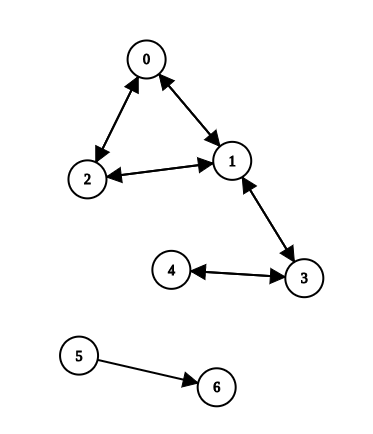
\includegraphics[width=.8\linewidth]{img/grafoesempio1.png}
			\caption{Grafo prodotto dal codice (a)}
	\end{subfigure}%
\end{figure}
\ \\
Il tipo \lstinline[style=cmd]|grafo| è definito in \lstinline[style=cmd]|graphUtils| nel seguente modo:

\begin{lstlisting}[style=caml]
	type grafo = Grafo of (int -> int list);;
\end{lstlisting}

\subsection{Data}
\subsubsection{.ml}

\subsection{Printer}

\subsection{GraphUtils}

\subsection{Main}

\subsection{Makefile}

File utilizzato per la compilazione del progetto che avviene tramite il comando \lstinline[style=cmd]|make|. 
Qualora un file venga modificato, questo permette di non dover ricompilare tutto il progetto ma solo quello che è stato cambiato. In una prima fase compila tutti i file \lstinline[style=cmd]|.ml| con i relativi \lstinline[style=cmd]|.mli|, generando 2 altri file:

\begin{itemize}
	\item \lstinline[style=cmd]|.cmi|: interfacce compilate utili per il corretto funzionamento dell'estensione \textit{OCaml} in \textit{Visual Studio Code} e per la corretta compilazione degli altri file.
	\item \lstinline[style=cmd]|.cmo|: file oggetto che verranno poi spostati nella cartella \lstinline[style=cmd]|build| per essere utilizzati nella fase di \textit{linking}
\end{itemize}
\ \\
Quindi, ogni file \lstinline[style=cmd]|.cmo| dipende dai relativi file \lstinline[style=cmd]|.ml| e \lstinline[style=cmd]|.mli|.
Successivamente, avvia la fase di \textit{linking} unendo insieme tutti i file \lstinline[style=cmd]|.cmo| e generando l'eseguibile \lstinline[style=cmd]|exe| nella cartella \lstinline[style=cmd]|bin|. All'interno di quest'ultima copia anche lo script python per permettere il corretto funzionamento del progetto.

\begin{lstlisting}[style=make, caption={Breve estratto del file Makefile}]
cc = ocamlc
cflags = -c
cinclude = -I src

srcdir = src
buildir = build
bindir = bin

target = $(bindir)/exe

.PHONY: clear

all: cartelle $(target)


$(target): 
	$(buildir)/graphUtils.cmo $(buildir)/printer.cmo 
	$(buildir)/data.cmo $(buildir)/main.cmo
		$(cc) -o $@ $^
		cp $(srcdir)/rappresentazione_grafo/rappresentazione_grafo.py $(bindir)

\end{lstlisting}
\section{Dimostrazione}
%TODO: aggiungere foto e mostrare come funziona in pratica il progetto.





